\documentclass[11pt,a4paper]{article}
\usepackage[T1]{fontenc}
\usepackage[utf8]{inputenc}
\usepackage{mathptmx}            % Times (scalable Type 1)
\usepackage[scaled=0.92]{helvet}
\usepackage{courier}
\usepackage[margin=2.4cm]{geometry}
\usepackage{microtype}
\usepackage{booktabs}
\usepackage{tabularx}
\usepackage{xcolor}
\usepackage{listings}
\usepackage{tikz}
\usetikzlibrary{arrows.meta,positioning}
\usepackage{enumitem}
\usepackage[hidelinks]{hyperref}

\lstset{basicstyle=\ttfamily\small,columns=fullflexible,frame=single,breaklines=true,
        backgroundcolor=\color{black!3},rulecolor=\color{black!20}}
\setlist{itemsep=2pt,topsep=4pt}
\setlength{\emergencystretch}{3em}

\title{\textbf{VaporPkg}: Blocking AI-Hallucinated and Suspicious\\ Package Installs at the Command Line}
\author{Varshith\\ \small Blekinge Institute of Technology (BTH), Sweden}
\date{October 2026}

\begin{document}
\maketitle

\begin{abstract}
Code-generating large language models (LLMs) frequently recommend software packages that do not exist.
Because public registries such as PyPI and npm let anyone claim an unused name, an attacker who registers
a frequently hallucinated name can deliver malware to every developer who copies the suggested install
command, an attack now called \emph{slopsquatting}. This report presents VaporPkg, a dependency-free
command-line guard that intercepts \texttt{pip}, \texttt{uv}, \texttt{poetry}, \texttt{npm}, \texttt{pnpm},
\texttt{yarn}, \texttt{bun} and \texttt{npx}-style commands, extracts every package they would fetch, and
scores each one with explainable signals: existence, registry quarantine status, malicious-package
advisories, package age, release history, lookalike similarity to popular names, install-time scripts and
provenance metadata. On live registries, VaporPkg raised no alerts on 600 sampled popular packages and
warned on 6--9\,\% of long-tail packages, which are mostly new or single-release projects. It also ships
a reproducible benchmark that measures hallucination rate and \emph{persistence} of hallucinated names
across models.
\end{abstract}

\section{Introduction}
LLM coding assistants are now part of everyday development. When asked for code that needs a third-party
library, they often answer with an install command such as \texttt{pip install <name>}. Spracklen et
al.~\cite{spracklen} generated 576{,}000 code samples with 16 models and found that 19.7\,\% of recommended
packages did not exist (5.2\,\% for commercial models, 21.7\,\% for open models), with over 200{,}000
unique hallucinated names. Many of those names recurred when the same prompt was repeated, which makes them
predictable. Security researchers have demonstrated the attack in practice by registering a hallucinated
name (\texttt{huggingface-cli}) as an empty package and observing thousands of real downloads~\cite{lasso}.

Classic typosquatting defences~\cite{spellbound} assume the victim mistypes a \emph{popular} name.
Hallucinated names are different: they are often plausible compositions (\texttt{flask-jwt-simple-auth})
far from any single popular package, so edit-distance checks alone miss them. The most reliable signal is
also the simplest one: \emph{the name does not exist yet}, or it was registered very recently.

\paragraph{Contributions.}
\begin{enumerate}
  \item A guard that sits in front of 13 package-manager entry points and refuses to execute installs of
        non-existent, quarantined, malicious or high-risk packages, with transparent per-signal reasons.
  \item A parser that extracts install candidates from shell commands, dependency files
        (requirements files, \texttt{pyproject.toml}, \texttt{package.json}) and free text such as
        LLM answers, including \texttt{import}/\texttt{require} statements with import-to-distribution
        mapping.
  \item A reproducible benchmark harness for package hallucination (rate, persistence, cross-model overlap)
        and an alert-rate study on real registry data.
\end{enumerate}

\section{Threat model}
The attacker can register any unclaimed name on PyPI or npm, publish arbitrary code (including npm
install scripts or Python build hooks that run at install time), and choose names that LLMs are likely to
produce. The attacker cannot modify the registries themselves or existing packages owned by others
(account takeover of popular packages is out of scope, but known malicious versions are surfaced via OSV).
The victim is a developer or CI pipeline that installs packages suggested by an LLM without verifying them.
VaporPkg's goal is to stop the install \emph{before} any attacker code runs, at negligible cost for
legitimate, established packages.

\section{Design}
\begin{figure}[h]
\centering
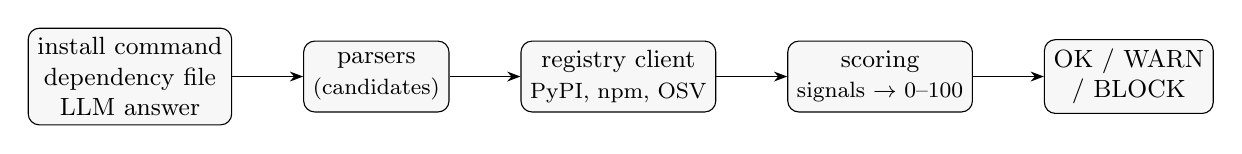
\begin{tikzpicture}[node distance=0.55cm and 0.9cm, box/.style={draw,rounded corners,align=center,
  font=\small,minimum height=0.9cm,fill=black!3}, >={Stealth}]
\node[box] (in) {install command\\ dependency file\\ LLM answer};
\node[box,right=of in] (p) {parsers\\ \footnotesize(candidates)};
\node[box,right=of p] (r) {registry client\\ \footnotesize PyPI, npm, OSV};
\node[box,right=of r] (s) {scoring\\ \footnotesize signals $\to$ 0--100};
\node[box,right=of s] (v) {OK / WARN\\ / BLOCK};
\draw[->] (in)--(p); \draw[->] (p)--(r); \draw[->] (r)--(s); \draw[->] (s)--(v);
\end{tikzpicture}
\caption{VaporPkg pipeline. Lookups run in parallel and are cached (24\,h; 1\,h for missing names).}
\end{figure}

\subsection{Candidate extraction}
Install commands are tokenised with shell-aware splitting that stops at control operators
(\texttt{\&\&}, \texttt{;}, \texttt{|}) and comments, and handles chained commands on one line, IPython
magics (\texttt{\%pip}) and runners (\texttt{npx}, \texttt{uvx}, \texttt{pipx run}), where only the
executed package is relevant. Requirement strings follow PEP~508; direct URL references, local paths,
wheels and VCS URLs are skipped because they are not resolved from the public index. npm aliases
(\texttt{"x": "npm:real@1"}) resolve to the real name; GitHub shorthands and \texttt{file:}/\texttt{link:}
specifiers are skipped. Candidates found only via \texttt{import} statements are marked low-confidence:
standard-library modules (\texttt{sys.stdlib\_module\_names}) and Node built-ins are removed, and about 90
common import$\to$distribution mismatches (\texttt{cv2}$\to$\texttt{opencv-python}) are mapped.

\subsection{Registry evidence}
For PyPI the JSON API provides releases with upload times, project URLs and ownership (including
organization accounts). When the JSON API returns 404, the Simple API (PEP~691) distinguishes three cases:
the name is unregistered, it is registered but has no installable files, or it carries a PEP~792 status
such as \texttt{quarantined}. For npm the full packument provides creation time, versions, repository,
maintainers and install scripts; popular packages are fetched with the abbreviated install metadata to save
bandwidth, in which case age and provenance signals are not computed. npm security placeholders
(\texttt{0.0.1-security}) are detected. Optionally, OSV is queried for OpenSSF \texttt{MAL-*} advisories,
and weekly download counts are fetched for non-popular packages.

\subsection{Scoring}
Each signal contributes points (Table~\ref{tab:signals}); critical signals block outright. The default
policy blocks at $\geq 70$ and warns at $\geq 30$. Packages in the top-15{,}000 download lists are capped
at 20 points unless a critical signal fires, because popular packages legitimately have install scripts or
few maintainers. Missing names derived only from imports produce a warning instead of a block.

\begin{table}[h]
\centering\small
\begin{tabularx}{\linewidth}{@{}>{\raggedright\arraybackslash}p{5.6cm} r >{\raggedright\arraybackslash}X@{}}
\toprule
Signal & Points & Rationale \\ \midrule
NOT\_FOUND, QUARANTINED, SECURITY\_HOLDING, KNOWN\_MALICIOUS & block & Hallucinated or removed-for-malware names. \\
VERY\_NEW ($<$14 d) / NEW ($<$90 d) & 45 / 25 & Squats are registered shortly before exploitation. \\
LOOKALIKE & 35 / 20 & $\leq$1--2 edits (optimal string alignment) from a top-5{,}000 name; separator confusion; popular name plus affix. \\
SINGLE\_RELEASE / FEW\_RELEASES & 15 / 8 & No maintenance history. \\
VERY\_LOW / LOW\_DOWNLOADS & 20 / 10 & $<$50 / $<$1{,}000 weekly downloads. \\
INSTALL\_SCRIPTS & 15 & npm pre/post-install hooks execute code. \\
NO\_REPOSITORY / NO\_DESCRIPTION & 12 / 8 & Weak provenance. \\
DEPRECATED & 10 & Abandoned or archived. \\
VERIFIED\_ORG & $-10$ & PyPI organization ownership. \\ \bottomrule
\end{tabularx}
\caption{Risk signals and default weights.}\label{tab:signals}
\end{table}

\section{Evaluation}
\subsection{Correctness}
An offline test suite (30 tests, fake registry transport) covers PEP~508 edge cases, nested
requirement files with hashes and line continuations, \texttt{pyproject.toml} (PEP~621, PEP~735 dependency
groups, Poetry), \texttt{package.json} aliases, pip/npm option parsing, extraction from a realistic LLM
answer, all verdict paths, caching, SARIF output and the guard's refusal to execute blocked installs.

\subsection{Alert rates on real packages}
To quantify the cost of the policy for legitimate users, VaporPkg was run against live registries on
2026-10-05 (seed 7) for four cohorts (Table~\ref{tab:alerts}). The OSV and download-count endpoints were
unreachable from the measurement environment, so those two signals were disabled. All other signals were
computed from live data.

\begin{table}[h]
\centering\small
\begin{tabular}{@{}lrrrrr@{}}
\toprule
Cohort & $n$ & OK \% & WARN \% & BLOCK \% & Median lookup \\ \midrule
Popular PyPI (top-15k sample) & 300 & 100.0 & 0.0 & 0.0 & 30 ms \\
Popular npm (top-15k sample) & 300 & 99.7$^*$ & 0.0 & 0.0 & 57 ms \\
Random PyPI (outside top 15k) & 300 & 91.3 & 6.0 & 2.7 & 29 ms \\
Long-tail npm (outside top 15k) & 300 & 90.7 & 9.3 & 0.0 & 90 ms \\ \bottomrule
\end{tabular}
\caption{Verdict distribution on existing packages. $^*$One transient network error (now retried).}\label{tab:alerts}
\end{table}

Popular packages produced no alerts. In the uniform random PyPI sample, every BLOCK (8 of 300) was a
registered name with \emph{no installable files} (deleted or placeholder projects). Installing those fails
anyway, and whoever controls the name could publish code under it later. Warnings in the long tail were
dominated by \textsc{new}, \textsc{single\_release} and \textsc{no\_repository}. These are not necessarily
false positives, since unvetted new packages are exactly the risk class, but they show the friction of the
policy. That friction is why WARN prompts the user instead of blocking. Lookalike warnings on short
names motivated restricting edit-distance targets to names of at least five characters.

\subsection{Package-hallucination benchmark (protocol)}
The harness issues 70 coding tasks (40 Python, 30 JavaScript) to any OpenAI-compatible endpoint, by default
with three repetitions at temperature 0.7, and measures for each model and language: (i) mention-level and
unique-name hallucination rate, (ii) share of answers with at least one hallucinated package,
(iii) \emph{persistence}, meaning the fraction of (task, hallucinated name) pairs that recur in at least
two repetitions, (iv) suggested names that exist but are younger than 90 days (possible squats already
registered), (v) cross-model overlap, and (vi) the fraction of hallucinated names VaporPkg blocks.
By construction (vi) is 100\,\% for names that do not exist; the interesting quantities are (i)--(v).

\begin{table}[h]
\centering\small
\begin{tabular}{@{}lrrrr@{}}
\toprule
Model & Unique-name rate & Answer rate & Persistence & Recent existing \\ \midrule
\multicolumn{5}{@{}l}{\emph{Fill in from \texttt{bench/results/summary.md} after running the benchmark.}} \\
\bottomrule
\end{tabular}
\caption{Hallucination benchmark results (to be produced with \texttt{run\_bench.py} + \texttt{evaluate.py}).}
\end{table}

\section{Limitations and ethics}
VaporPkg raises the cost of slopsquatting but is not a malware scanner: a patient attacker can age a
package, add a repository link and inflate downloads. It should complement content scanners and
lockfile-based workflows. Lookalike detection depends on snapshot popularity lists, and private indexes are
not queried. For ethical reasons, raw lists of hallucinated names produced by the benchmark should not be
published. They should instead be reported to the registry security teams so the names can be reserved
or monitored.

\section{Conclusion}
A small amount of registry metadata, evaluated at the moment of installation, stops the most direct form
of slopsquatting (installing a name that does not exist or was just registered) with no measurable impact
on popular dependencies and a modest, explainable warning rate on the long tail.

\begin{thebibliography}{9}
\bibitem{spracklen} J.~Spracklen, R.~Wijewickrama, A.~H.~M.~N.~Sakib, A.~Maiti, B.~Viswanath, and
  M.~Jadliwala. ``We Have a Package for You! A Comprehensive Analysis of Package Hallucinations by Code
  Generating LLMs.'' \emph{USENIX Security Symposium}, 2025. arXiv:2406.10279.
\bibitem{lasso} B.~Lanyado. Research on AI package hallucinations and the \texttt{huggingface-cli}
  experiment. Lasso Security, 2024.
\bibitem{spellbound} M.~Taylor, R.~Vaidya, D.~Davidson, L.~De~Carli, and V.~Rastogi. ``Defending Against
  Package Typosquatting.'' \emph{Network and System Security (NSS)}, 2020.
\bibitem{ohm} M.~Ohm, H.~Plate, A.~Sykosch, and M.~Meier. ``Backstabber's Knife Collection: A Review of Open
  Source Software Supply Chain Attacks.'' \emph{DIMVA}, 2020.
\bibitem{pep792} PEP 792 -- Project status markers in the simple index. Python Software Foundation, 2025.
\bibitem{ossf} OpenSSF Malicious Packages repository. \url{https://github.com/ossf/malicious-packages}.
\end{thebibliography}
\end{document}
